\documentclass[10pt]{article}
\usepackage[letterpaper,margin=0.76in]{geometry}
\usepackage[T1]{fontenc}
\usepackage{lmodern}
\usepackage{microtype}
\usepackage{amsmath,amssymb}
\usepackage{booktabs}
\usepackage{graphicx}
\usepackage{float}
\usepackage{tikz}
\usetikzlibrary{arrows.meta,positioning}
\usepackage{enumitem}
\usepackage{natbib}
\usepackage{xcolor}
\usepackage{hyperref}
\usepackage{cleveref}
\hypersetup{
  colorlinks=true,
  linkcolor=blue!45!black,
  citecolor=blue!45!black,
  urlcolor=blue!55!black,
  pdftitle={Throughput Is Not Liveness: Three Clocks for GPU-Free Music Generation on iPhone},
  pdfauthor={Matt Mireles},
  pdfkeywords={on-device inference, generative audio, Core ML, Apple Neural Engine, real-time systems}
}
\setlist{nosep,leftmargin=1.45em}
\setlength{\emergencystretch}{2em}
\setlength{\parskip}{0.20em}
\setlength{\parindent}{1.1em}
\definecolor{aneBlue}{HTML}{0072B2}
\definecolor{cpuOrange}{HTML}{E69F00}
\title{\textbf{Throughput Is Not Liveness:}\\
Three Clocks for GPU-Free Music Generation on iPhone}
\author{Matt Mireles\\Independent Researcher\\\href{https://github.com/mattmireles}{github.com/mattmireles}}
\date{July 2026}
\begin{document}
\maketitle
\begin{abstract}
Real-time generative audio is usually reduced to one question: can inference run faster than playback? That criterion is necessary and insufficient. A system may average faster than real time while buffering tens of seconds of stale audio, and it may deliver every sample while a state-boundary error changes the sound. We present an end-to-end deployment and falsification study of the 230-million-parameter \texttt{\detokenize{mrt2_small}} live-music model on iPhone. The system combines a 12-layer temporal transformer, a 12-level residual-vector-quantized depth rollout, SpectroStream decoding, inverse STFT, and 48 kHz stereo delivery. A pure fixed-shape temporal graph executes on the Apple Neural Engine (ANE), while Swift owns its 41-frame K/V ring. Ten of ten cold processes admit the graph on both A17 Pro and A14, and a model-attributed trace contains temporal and decoder ANE work with no application-attributed GPU interval.

On an iPhone 15 Pro Max, the corrected runtime sustains 610 seconds in the foreground, reaches the \texttt{\detokenize{serious}} thermal state, completes 628 nominal one-second producer iterations in 609.65 seconds, and records zero underruns or drops. The p99 of iteration-normalized active stage cost is 24.81 ms per token against a 40 ms throughput budget. We emphasize what this number is not: it is the p99 of 25-token iteration means, not per-token tail latency. Backpressure bounds the queue near 21 seconds, so the experiment proves continuous throughput, not low-latency steering. Separate device evidence measures controller application in 4-15 ms but audible changes only after 6.48-9.02 seconds without queue discard. A final-code post-ring experiment then tests 30 matched-noise control resets with a five-frame decoder and a 160 ms retained queue. It completes 600 seconds with zero delivery or proof faults, but its frozen paired-reference detector misses 22 transitions; among eight detections, end-to-end p95 is 0.947 seconds. The attained deployment tier is therefore buffered, not responsive or live.

The first scientific result comes from a reviewer-motivated 2x2 crossover. For three seeds, we generate 600-second token trajectories with MLX and the shipped Core ML port, then decode each through stateful MLX or the stateless phone boundary. Fixed-token graph and DSP controls separate sampling, numerical, windowing, and reconstruction hypotheses. The pulse excess follows stateless decoder windowing in all 60 paired 30-second windows: median seed effect +0.01706, compared with +0.00018 for the Core ML graph itself. A direct tensor probe shows that the original 25-token calls discard causal convolution history; retaining 12 token frames raises correlation with stateful MLX from 0.108 to above 0.999999999. Adding that context reduces pulse share by 0.01650 and changes the original diagnostic-limit count from 35/60 windows to 13/60, versus 11/60 for stateful MLX. A new 600-second iPhone capture matches the stateful reference count at 5/20 windows for the principal seed, with no dropout. Thus the measured pulse excess first framed as long-horizon model degeneration was a systems boundary bug. A separate frozen liveness test then removes the ten-second temporal reset. Across three 600-second seeds, all three unrefreshed trajectories emit float-PCM samples at or above full scale; matched ten-second reset arms emit none. A K/V-only versus feedback-only factorial does not identify a unique causal state. Event-centered calibrated model votes reject 7/9 unrefreshed clips, whereas one blinded human engineering check finds both conditions technically acceptable in a late window that excludes the measured event and correctly rejects a corruption control. We therefore retain reset as an explicit bounded-trajectory protocol, not a model repair. The broader lesson is methodological: live generation has separate compute, delivery, and generative clocks, and a credible study must localize failures across all three without turning a detector into a causal claim.

\end{abstract}

\section{Introduction}
Live music generation is an unusually unforgiving systems workload. Its autoregressive model must keep producing, its audio callback must never wait, steering should become audible while the intent is still relevant, and the trajectory must remain musically plausible. A batch generator can finish late. A live generator that finishes late clicks or falls silent; one that buffers too aggressively plays an obsolete decision; one with incorrect state can run perfectly on time while sounding wrong.

Magenta RealTime introduced continuously steerable causal music generation \citep{live-music-models}. Magenta RealTime 2 (MRT2) provides open weights and an MLX implementation for Apple Silicon Macs \citep{mrt2}. Its small configuration emits 12 residual-vector-quantized (RVQ) codes at 25 Hz, and a SpectroStream decoder reconstructs 48 kHz stereo audio \citep{mrt2-model-card}. This paper asks whether the complete loop can execute continuously on an iPhone without application GPU work, and, more importantly, what evidence is needed to make that statement mean anything.

Our first answer conflated two failures. A signed A17 Pro runtime sustained 610 seconds with zero underruns and a growing reservoir. Its captured audio nevertheless crossed a predeclared 4-16 Hz envelope-pulse threshold and failed three of five exploratory automated listening votes. We reported a failed "generative clock." That causal framing did not survive the decisive token-by-decoder crossover: the measured pulse excess followed decoder windowing. But the correction did not establish indefinite model stability; the deployed runs still reset temporal state every ten seconds.

We therefore freeze three causal hypotheses for the pulse defect. H1 is model-intrinsic or sampling-induced recurrence: the pulse should follow tokens into either decoder. H2 is numerical divergence in the temporal/depth port: the Core ML token source should be worse after decoding with clean MLX. H3 is a decoder or DSP boundary error: the pulse should follow the stateless phone decoding path for either fixed token source. We then split H3 into an MLX FLOAT32 pre-iSTFT graph, the Core ML FP16 graph, the production C++ reconstruction core, and a measured context intervention. The result strongly supports a refined H3: a stateless causal decoder was invoked with insufficient left context. We then test the separate question the crossover cannot answer: whether an unrefreshed trajectory satisfies a frozen 600-second liveness contract.

This correction changes the paper's thesis. "Faster than playback" is not a complete real-time claim, and a failed audio detector is not a causal label. We define three clocks:

\begin{enumerate}
\item \textbf{Compute clock.} Sustained production rate must be at least playback rate. Batch-normalized stage costs describe headroom but do not become per-token tail latency by division.
\item \textbf{Delivery clock.} The callback must observe zero underruns and producer drops, while queued audio remains inside a band whose upper bound is chosen from an audible steering-latency budget.
\item \textbf{Generative clock.} Prompt-conditional audio measures and controlled comparisons must remain valid across the horizon. A detector can identify a symptom; only an intervention or crossover can identify its source.
\end{enumerate}
We make five contributions:

\begin{itemize}
\item A complete GPU-free placement and sustained-throughput study of MRT2 on A17 Pro, with a pure temporal graph, host-owned K/V state, in-process admission gates, and model-attributed accelerator evidence.
\item A duration-controlled thermal result: an A17 CPU+GPU-policy control has 38.51 ms p99 iteration-normalized cost in five short processes, but 49.23 ms over a matched 610-second run and crosses 40 ms only after minute six.
\item A three-seed, long-horizon token-by-decoder crossover that localizes a plausible generative failure to missing causal decoder history, plus a 12-frame overlap intervention verified at tensor, audio, and physical-device levels.
\item A frozen unrefreshed liveness experiment in which no-reset fails an objective float-PCM full-scale gate in 3/3 seeds, matched reset passes in 3/3, and a state-reset factorial honestly terminates at ambiguous attribution.
\item A corrected delivery contract that distinguishes continuous playback from interactive steering, plus a complete post-ring A17 Pro falsification: the final code delivers 600 seconds and 30 transitions without faults, yet a frozen paired-reference detector misses 22 changes and measures 0.947-second p95 among eight detections, so the runtime remains buffered.
\end{itemize}
The weights are unchanged. Previous conversion and accelerator-admission findings appear in the companion \emph{Surgical Inference} manuscript \citep{surgical-inference}. Here the units of contribution are the composed runtime, sustained physical-device evidence, causal audio localization, and measurement contract.


\begin{align}
\mathcal{C}_{\mathrm{compute}} &\equiv R_{\mathrm{producer}} \ge 1, \\
\mathcal{C}_{\mathrm{delivery}} &\equiv
  (U=0) \land (D=0) \land (0 < B(t) \le B_{\max}), \\
\mathcal{C}_{\mathrm{gen}} &\equiv \bigwedge_{k=1}^{K} m_k \in \mathcal{A}_k.
\end{align}
Here $R_{\mathrm{producer}}$ is sustained generated-audio rate relative to
playback, $U$ and $D$ are callback underruns and producer drops, $B$ is queued
PCM, and $B_{\max}$ is chosen from an audible steering-latency budget. Each
$m_k$ is a prompt-conditional audio measure with acceptance set $\mathcal{A}_k$.
No score from one clock substitutes for another.

\section{Background and related work}
\subsection{Live music and neural audio}
MusicGen generates text- or melody-conditioned music from interleaved codec tokens \citep{musicgen}. RAVE demonstrated 48 kHz neural synthesis faster than real time on a laptop CPU \citep{rave}. Live Music Models instead make causality and continuous steering part of the product contract \citep{live-music-models}. MRT2 is the open model used here. Its SpectroStream codec operates in the time-frequency domain and supports full-band stereo \citep{spectrostream}, extending the streamable neural-codec lineage of SoundStream and EnCodec \citep{soundstream} \citep{encodec}.

Autoregressive generation can amplify model or decoding errors over a long horizon \citep{next-token-barrier}. Repetitive text degeneration motivated dynamic nucleus sampling \citep{neural-text-degeneration}. These results make recurrence a credible hypothesis for a periodic audio symptom, not a conclusion. In our case, both MLX and Core ML trajectories retain full distinct-frame ratio, about 6.2-6.4 bits of mean per-level entropy in late complete windows, and no exact period-1 through period-8 cycles. More decisively, the symptom follows decoder windowing under fixed tokens.

\subsection{Mobile heterogeneous inference}
MLPerf Mobile emphasizes that on-device performance is a property of the full software-hardware stack \citep{mlperf-mobile}. Apple documents fixed-shape transformer deployment patterns for the ANE \citep{apple-ane-transformers,coremltools}. Similar heterogeneous scheduling appears in mobile NPU work such as \texttt{\detokenize{llm.npu}} \citep{llm-npu}. MRT2 differs from mobile LLM prefill: it repeats a small causal step indefinitely, feeds an audio callback, and exposes every state or timing error to a listener. Requested compute units, graph conversion, and a short latency benchmark are therefore weak proxies. We separately measure admission, accelerator activity, sustained capacity, callback continuity, queue depth, and audio behavior.

\section{System design}
\subsection{Workload and host boundary}
At 25 Hz, one MRT2 token frame represents 1,920 output samples and 40 ms of 48 kHz stereo audio. The temporal transformer has 12 layers and consumes the previous frame's mean token embedding, source conditioning, and a local attention history. The depth transformer autoregressively selects 12 RVQ codes. Their 256-dimensional codebook rows are summed and passed to the SpectroStream decoder. \cref{fig:system} shows the deployed boundary.

The temporal graph is a pure single-frame tensor function. Inputs contain the current temporal and source vectors, a fixed-shape validity bias, and 48 ordinary K/V arrays for self- and cross-attention across 12 layers. Outputs contain one temporal vector and 48 one-token cache updates. Swift owns a preallocated 41-frame chronological ring. This removes in-graph state mutation, which had compiled in a probe but failed ANE admission in the application.

The state proof asks two independent questions. First, identical input on fresh and warmed state must diverge, preventing a write-only-state false pass. Second, 64 consecutive predictions must match a frozen reference, including 23 after the ring wraps. Correlation is 0.9995 on both phones, and all outputs are finite. The runtime repeats this proof and queries the temporal compute plan at session start.

\subsection{One-call depth rollout}

\begin{table}[H]
\centering
\small
\caption{Measured A14 depth rollout ablation. The in-graph boundary removes host
boundaries but still traverses transformer weights at each dependent RVQ level;
the major gain is FLOAT16, not a fictitious single weight traversal.}
\label{tab:depth}
\begin{tabular}{@{}lrr@{}}
\toprule
Depth boundary & Precision & ms/token frame \\
\midrule
12 separate full-pass predictions & FLOAT32 & 40.2 \\
One in-graph 12-level prediction & FLOAT32 & $\sim$37.0 \\
One in-graph 12-level prediction & FLOAT16 & 12.7 \\
\bottomrule
\end{tabular}
\end{table}

The depth transformer has dependent RVQ levels: level \texttt{\detokenize{k+1}} consumes the code selected at level \texttt{\detokenize{k}}. Twelve separate Core ML predictions on A14 cost 1,004 ms per 25-frame producer iteration, or 40.2 ms per token frame. A one-prediction graph unrolls the dependency, takes host-generated Gumbel noise, applies the fixed top-40 mask, gathers embeddings, and returns all 12 codes plus temporal feedback.

The measured ablation corrects an easy but false bandwidth story. The in-graph rollout does not turn 12 dependent transformer applications into one weight traversal. FLOAT32 still costs about 37 ms per frame. The large gain comes from the validated FLOAT16 artifact, which measures 12.7 ms on A14 and 8.4 ms on A17 Pro (\cref{tab:depth}). FLOAT32 is token-exact in 900 comparisons; FLOAT16 flips near-tie tokens and was accepted only after distributional and device audio gates.

\subsection{Decoder context and reconstruction}
The original phone decoder accepted 25 token embeddings and emitted 96 STFT frames. The host advanced by 24 token frames, preserving only the one-frame SpectroStream lookahead. This treated the decoder as a finite-window function. Its convolutional stack is causal but stateful: output near a boundary depends on more history than the formal lookahead.

The corrected boundary retains 12 token frames. The first 25-token prediction initializes reconstruction state and emits its full 96 STFT frames. Each later prediction advances by 12 tokens, drops the first 48 context STFT frames, and emits the 48 new frames. The Core ML input shape and model artifact remain unchanged. A preallocated FLOAT32 crop buffer materializes logical output using the declared \texttt{\detokenize{MLMultiArray}} shape and strides; allocation and DSP remain off the audio callback.

The C++ inverse STFT uses the periodic Hann synthesis window used by upstream SpectroStream and performs overlap-add into a lock-free single-producer, single-consumer PCM ring. During diagnosis we found a second parity debt: the old C++ core applied a normalized dual-window convention. Direct sample tests now match the upstream periodic-Hann reconstruction. However, this change alone \emph{increases} pulse share by a median 0.00321 across seeds. It is a real parity fix but not the causal fix for the reported symptom.

\subsection{Buffering and steering}
Inference and reconstruction run on a producer task. The Core Audio callback only reads a bounded ring and zero-fills an underflow. A startup reservoir absorbs jitter. Once the ring reaches its high watermark, producer backpressure prevents unbounded memory growth.

That architecture guarantees neither low latency nor liveness. A high watermark of roughly 21 seconds allows 21 seconds of already-rendered intent. In an earlier two-event control test, the controller applied new state after 0.015 and 0.004 seconds, but matched-reference audible changes arrived after 6.479 and 9.023 seconds. A proof-mode queue discard retained 19,200 frames (0.4 seconds), faded in over 3,840 frames, discarded 647,936 frames, and ended with zero underruns and drops. The capture point was before the playback ring, so that receipt cannot prove click-free speaker output. We therefore report continuous buffered playback as solved and subsecond audible steering as open.

The final steering harness moves the proof tap after ring discard and fade, so the stored PCM is the sequence offered to Core Audio. At each scripted control event it retains a bounded queue, applies a 40 ms fade, and resets temporal K/V plus previous-token feedback. For the proof only, every no-op and cross-class event restarts sampling from the same seed; this matched-noise design makes the no-op events calibrate the generic reset while target changes isolate conditioning. It is not the shipping sampling policy.

Two control-boundary bugs surfaced under this harness. First, a producer that awoke from backpressure could decode a window captured under the prior control epoch; the runtime now rechecks the epoch after the await and suppresses that stale emission. Second, suffix pruning retained one old lookahead embedding in addition to causal context, leaking 40 ms of prior-control PCM. The final policy retains exactly the decoder's two causal context frames. Focused regressions cover both boundaries; the complete device run below uses the corrected build.

\subsection{Ten-second temporal refresh}
All principal device and crossover trajectories reset temporal K/V and the previous-frame feedback vector every 10 seconds. Decoder context, overlap-add, and queued PCM remain continuous. This condition must be stated because the 41-frame ring covers only 1.64 seconds. After 10 seconds, attention slots have already rolled over several times; the intervention's distinctive long-horizon effect is resetting the recurrent feedback loop and returning the cache to a cold start. It is a deployed bounded-trajectory protocol here, not evidence that an unrefreshed model is stable.

The reset is deliberately not described as a fix. It changes both K/V history and recurrent feedback, thereby selecting a new autoregressive trajectory. A rare peak disappearing after an intervention demonstrates bounded operation; it does not, by itself, localize the mechanism or establish that every unrefreshed trajectory is perceptually defective.


\begin{figure}[t]
  \centering
  \resizebox{\textwidth}{!}{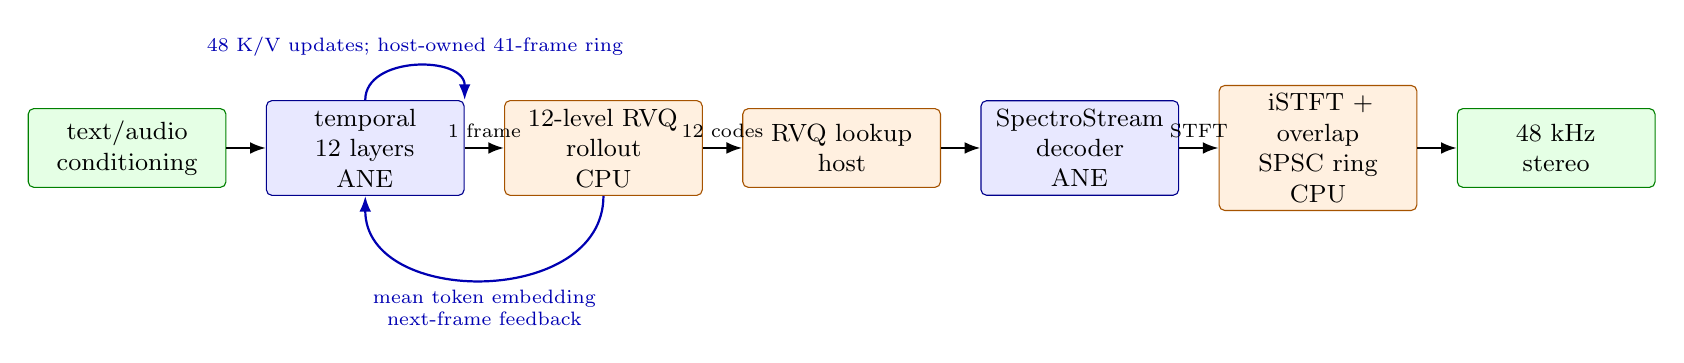
\begin{tikzpicture}[
  font=\small,
  node distance=6mm and 5mm,
  box/.style={draw, rounded corners=2pt, minimum height=10mm, text width=23mm, align=center, inner sep=3pt},
  ane/.style={box, fill=blue!9, draw=blue!55!black},
  cpu/.style={box, fill=orange!12, draw=orange!65!black},
  io/.style={box, fill=green!10, draw=green!50!black},
  arrow/.style={-{Latex[length=2mm]}, thick}
]
\node[io] (prompt) {text/audio\\conditioning};
\node[ane, right=of prompt] (temporal) {temporal\\12 layers\\ANE};
\node[cpu, right=of temporal] (depth) {12-level RVQ\\rollout\\CPU};
\node[cpu, right=of depth] (lookup) {RVQ lookup\\host};
\node[ane, right=of lookup] (decoder) {SpectroStream\\decoder\\ANE};
\node[cpu, right=of decoder] (render) {iSTFT + overlap\\SPSC ring\\CPU};
\node[io, right=of render] (audio) {48 kHz\\stereo};
\draw[arrow] (prompt) -- (temporal);
\draw[arrow] (temporal) -- node[above, font=\scriptsize] {1 frame} (depth);
\draw[arrow] (depth) -- node[above, font=\scriptsize] {12 codes} (lookup);
\draw[arrow] (lookup) -- (decoder);
\draw[arrow] (decoder) -- node[above, font=\scriptsize] {STFT} (render);
\draw[arrow] (render) -- (audio);
\draw[arrow, blue!70!black] (depth.south) to[out=-90,in=-90,looseness=1.2]
  node[below, font=\scriptsize, align=center] {mean token embedding\\next-frame feedback} (temporal.south);
\draw[arrow, blue!70!black] (temporal.north) to[out=90,in=90,looseness=1.15]
  node[above, font=\scriptsize, align=center] {48 K/V updates; host-owned 41-frame ring} (temporal.north east);
\end{tikzpicture}
}
  \caption{End-to-end deployment boundary. Blue stages are observed on the ANE;
  orange stages remain deliberate host/CPU work. Temporal recurrence crosses the
  model boundary as ordinary K/V tensors; the stateless decoder retains 12 token
  frames of measured causal context. No claim of an ``all-ANE'' system is made.}
  \label{fig:system}
\end{figure}

\section{Experimental method}
\subsection{Devices, artifacts, and placement}
The primary device is a 2023 iPhone 15 Pro Max (\texttt{\detokenize{iPhone16,2}}, A17 Pro). The boundary device is a 2020 iPhone 12 Pro (\texttt{\detokenize{iPhone13,3}}, A14). Signed release builds run in the foreground with the screen on. The fixed condition is \texttt{\detokenize{warm ambient texture}}, certified \texttt{\detokenize{warm.bin}} source conditioning, top-k 40, style guidance 3.1, temperature 1.0, and seed 20260718 unless a replication seed is named.

Placement has two receipts. Ten cold application processes query \texttt{\detokenize{MLComputePlan}}; all ten assign temporal estimated cost 1.0 to the ANE on each phone and pass the state proof. A process-targeted Instruments trace then records temporal and decoder ANE predictions, Core ML activity for every model family, and an empty application Metal GPU table. The claim is GPU-free, not all-ANE: depth, Gumbel generation, RVQ lookup, cache mutation, inverse STFT, ring management, logging, and UI work remain on the CPU.

\subsection{Throughput and the batch-normalized cost}
One producer iteration generates 25 temporal/depth frames and one to three decoder calls. We preserve the historical diagnostic

\[t_{\mathrm{eff}} = \frac{t_{\mathrm{temporal}} + t_{\mathrm{depth}} + t_{\mathrm{sampling}} + t_{\mathrm{decoder}}}{25}.\]
We rename it \textbf{iteration-normalized compute cost}. Its p99 is the p99 of a mean over each 25-token iteration. It suppresses within-iteration dispersion and cannot certify a per-token deadline. The actual compute-clock verdict is sustained nominal generated duration divided by producer wall time, combined with the delivery counters and ring trajectory. We still report the normalized quantiles because they decompose thermal changes and preserve comparison with the earlier campaign.

The final corrected A17 run lasts 610 seconds after audio start, captures 600 seconds of PCM, logs every producer iteration, and records token frames after warmup. A separate five-process campaign provides run-level medians and IQRs for temporal ANE and CPU+GPU requested policies. A matched 610-second CPU+GPU-policy run exposes duration effects.

\subsection{Crossover design}
For seeds 20260718, 271828, and 1618033, both the MLX sampler and an exact Python implementation of the shipped Core ML graph/host boundary generate 15,001 token frames, enough for 600 seconds after decoder lookahead. Each uses its native seeded random-number implementation; token-source arms are therefore independent trajectories, not token-by-token parity trials. Within every decoder comparison, however, the token file is fixed and hash-identical.

The principal 2x2 crosses token source (MLX or Core ML port) with decoder path (stateful streaming MLX or stateless Core ML plus C++ DSP). A fifth arm replaces only the Core ML decoder graph with the MLX FLOAT32 pre-iSTFT graph while preserving 25-token windows and C++ reconstruction. Four more arms cross both token sources and decoder graphs with the corrected periodic-Hann DSP. The causal intervention then repeats MLX and Core ML graphs with 12 frames of left context and identical corrected DSP.

For each 30-second window we measure the fraction of RMS-envelope spectral power from 4 to 16 Hz. The original 0.070 limit was frozen for one ambient prompt before this study. We retain it as a diagnostic count, not a universal music-quality boundary: legitimate rhythm occupies the same band. Primary inference uses paired effect sizes over all windows and reports the median and range of seed-level means. We do not treat 60 temporally adjacent windows as 60 independent samples.

\subsection{Frozen unrefreshed liveness protocol}
The liveness gate is fixed before replication: a candidate passes only if a 600-second float-PCM decode contains zero samples with \texttt{\detokenize{abs(x) >= 1.0}}. Because the stored path is floating point, crossing 1.0 is called \textbf{full-scale overrange}, not hard clipping; we separately inspect finiteness, saturation, dropout, token cycles, and perceptual evidence. The prompt, checkpoint, conditioning, temperature, top-k, decoder, DSP, and seeds are held fixed.

For each of seeds 20260718, 271828, and 1618033, a 2x2 reset factorial runs without reset, with K/V reset only, with previous-frame feedback reset only, and with both reset every ten seconds. RNG state and absolute position remain continuous. The predeclared decision requires a replicated no-reset failure and a consistent arm-level rescue; otherwise attribution is ambiguous and no new mitigation is selected. This is a trajectory intervention, not a paired-token ablation: resetting state changes subsequent sampled tokens.

Listening is supplemental. Three opaque event-centered lineups per seed contain a reset baseline, the unrefreshed candidate, and deterministic corruption control. Votes count only when the baseline passes and corruption fails. A separate blinded human engineering check uses a presealed late 30-second window; it is an instrument/control check, not a participant study or a substitute for full-trajectory measurement.

\subsection{Post-ring steering protocol}
Two class-reference events and four same-class no-op calibrations precede 30 alternating C-major/drums and C-minor/drumless transitions. For each class, the detector compares 20 ms post-event waveform frames against the matched-noise reference trajectory, allows 12 ms alignment, requires three consecutive 1 ms hops, and freezes its threshold as the largest false-target score in the no-op windows plus 0.02. A responsive pass requires end-to-end p95 at most 0.50 seconds and maximum at most 0.75 seconds; a live pass requires p95 at most 0.20 seconds and maximum at most 0.25 seconds. Any underrun, producer drop, proof-ring loss, full-scale sample, or missed transition fails promotion. The detector, 160 ms queue, transition schedule, and thresholds are frozen before the complete run; a failure blocks speaker/listening promotion rather than inviting post-hoc tuning.

\subsection{Independent evidence and receipts}
The decoder-context tensor probe compares a stateful MLX prefix against stateless 25-token evaluations at one fixed segment while varying retained history over 0, 1, 2, 4, 8, and 12 tokens. The production C++ reconstruction has an independent sample-level parity test against a NumPy periodic-Hann inverse STFT and overlap-add implementation.

Every public result is generated from a machine-readable receipt. The raw device WAVs, events, tokens, and traces behind those receipts are public (Artifact statement); their SHA-256 hashes, normalized summaries, commands, model identities, and source hashes were public from first submission and remain the verification path of record. Precision experiments stop in the order finite, deterministic parity, device latency, then audio; a wrong function never earns a favorable speed number.

\section{Results}

\begin{table}[H]
\centering
\small
\caption{Sustained foreground results. Cost is a p99 over 25-token iteration
means, not per-token tail latency. The corrected A17 runtime sustains throughput
and playback; its 21 s queue does not satisfy low-latency steering. The CPU+GPU
control and A14 rows predate the decoder-context repair and are conservative
duration/hardware controls.}
\label{tab:sustain}
\begin{tabular}{@{}lrrrrll@{}}
\toprule
Device & p50 & p90 & p99 & Rate & First underflow & Verdict \\
 & \multicolumn{3}{c}{iteration-normalized ms/token} & ($\times$RT) & & \\
\midrule
A17 ANE + context & 23.50 & 24.33 & 24.81 & 1.030 & none / 610 s & throughput pass \\
A17 CPU+GPU & 23.56 & 43.55 & 49.23 & 1.008 & none / 610 s & compute fail \\
A14 ANE & 43.88 & 47.25 & 58.59 & 0.897 & 294.08 s & fail \\
\bottomrule
\end{tabular}
\end{table}

\subsection{Reliable ANE admission and GPU absence}
Both devices pass 10/10 cold-process temporal admission and state gates. The A17 trace contains 653 temporal ANE predictions and 24 decoder ANE predictions, plus expected CPU depth activity. The application's Metal GPU table contains zero intervals and zero duration. The A14 cross-device trace reaches the same placement verdict. Moving recurrence to ordinary tensor I/O therefore makes admission repeatable in the application without deleting transformer math.

\subsection{Sustained A17 throughput, with the metric named honestly}
The corrected A17 context-12 runtime completes 628 nominal one-second producer iterations over 609.65 seconds of producer-loop wall time, a 1.030x nominal rate. It reaches \texttt{\detokenize{serious}} thermal state and records zero callback underruns, zero producer drops, and no near-zero dropout longer than one sample. The PCM capture is exactly 600.0 seconds, finite, unclipped, and stereo. \cref{tab:sustain} summarizes the physical-device results.

Iteration-normalized stage cost is 23.50 ms p50, 24.33 ms p90, and 24.81 ms p99. Decoder context roughly doubles decoder cadence: decoder work rises to 58.74 ms per 25-token iteration at p50, while temporal and depth remain 280.01 and 246.14 ms. Backpressure occupies 38.9\% of producer-loop wall time, direct evidence that sustained capacity exceeds playback.

The delivery statement is narrower. Queue fill starts at 2.88 seconds, never falls below 2.73 seconds, and ends at 21.01 seconds, near the configured high watermark. That proves safe continuous playback for the measured run. It also quantifies why the default runtime is not a low-latency steering system.

\subsection{Duration changes the placement verdict}

\begin{table}[H]
\centering
\small
\caption{Independent-process pre-context latency campaign, five runs per cell. Entries are
median (IQR) across run-level percentiles. The CPU+GPU control changes only the
requested temporal policy; depth remains CPU and decoder remains ANE.}
\label{tab:dispersion}
\begin{tabular}{@{}llrrrr@{}}
\toprule
Device & Temporal & p50 & p99 & Temporal p50 & Startup \\
 & policy & \multicolumn{3}{c}{iteration-normalized ms/token} & s \\
\midrule
A17 Pro & ANE & 20.77 (.03) & 22.35 (.42) & 11.25 (.01) & 4.26 (.04) \\
A17 Pro & CPU+GPU & 27.32 (.25) & 38.51 (1.78) & 16.35 (.15) & 6.22 (.05) \\
A14 & ANE & 40.38 (1.00) & 50.72 (3.30) & 13.85 (.63) & 7.52 (.01) \\
A14 & CPU+GPU & 49.73 (1.11) & 50.64 (1.41) & 24.85 (.17) & 9.76 (.14) \\
\bottomrule
\end{tabular}
\end{table}


\begin{figure}[H]
  \centering
  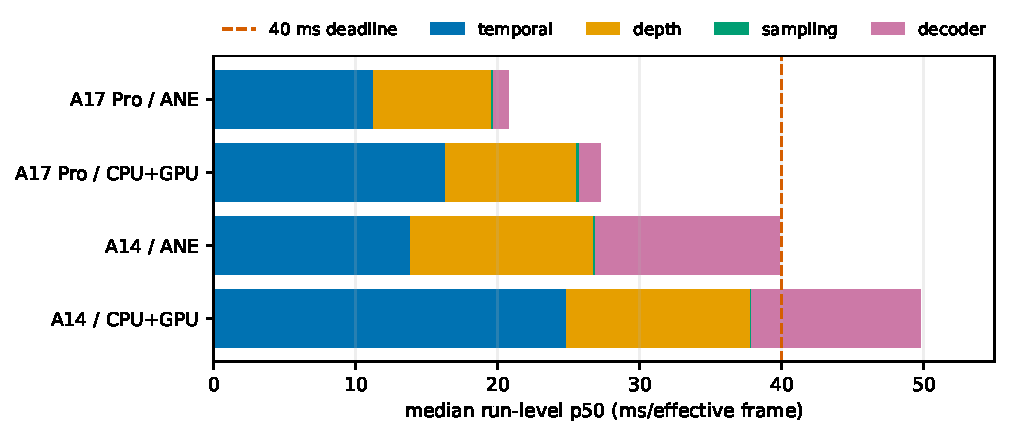
\includegraphics[width=0.94\textwidth]{figures/fig-latency.pdf}
  \caption{Stage decomposition for the repeated-process campaign. Bars use
  the median of run-level stage p50 values. The selected ANE policy reduces
  temporal cost on both phones. These are quantiles of iteration means, not
  per-token latency quantiles. CPU+GPU denotes a requested Core ML policy, not
  a GPU-placement proof.}
  \label{fig:latency}
\end{figure}


\begin{figure}[H]
  \centering
  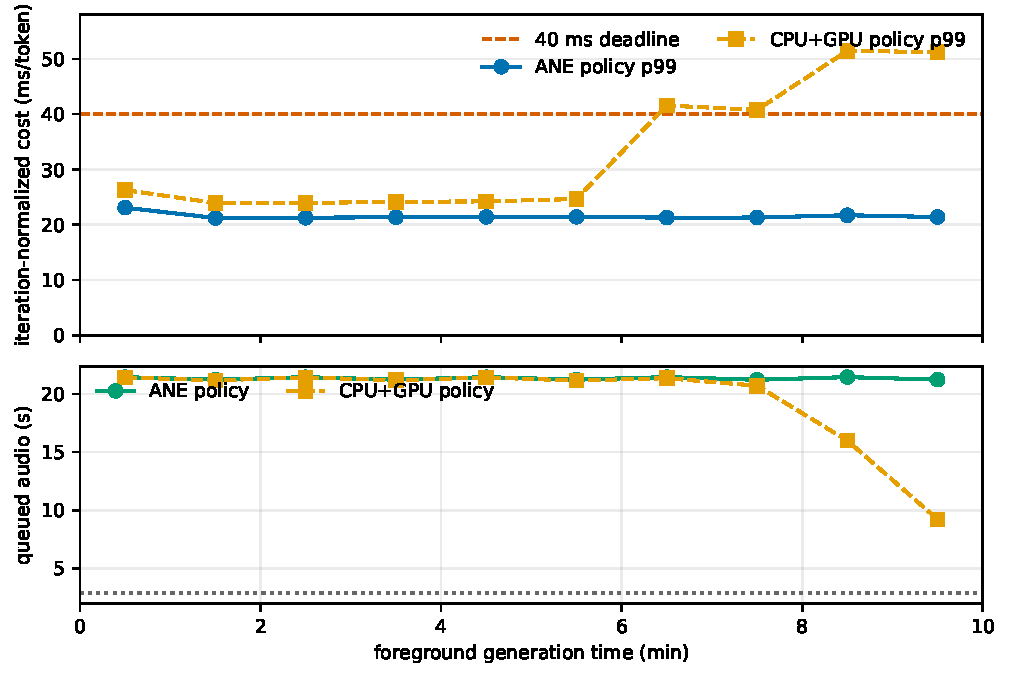
\includegraphics[width=0.94\textwidth]{figures/fig-soak.pdf}
  \caption{A17 Pro matched pre-context ten-minute trajectories. The selected
  ANE-policy run keeps iteration-normalized p99 flat. The CPU+GPU-policy control
  moves from 38.51 ms in five short processes to 49.23 ms here and crosses 40 ms
  after minute six. The duration effect is visible even though buffering prevents
  an underrun.}
  \label{fig:soak}
\end{figure}

The five-process pre-context campaign reports A17 median run-level p99 iteration-normalized cost of 22.35 ms for temporal ANE and 38.51 ms for the CPU+GPU requested-policy control (\cref{tab:dispersion}, \cref{fig:latency}). In the matched 610-second control, the latter becomes 49.23 ms. Its per-minute p99 crosses 40 ms only after minute six and reaches 51.46 ms, while a banked reservoir drains from about 21 seconds to 7.65 seconds (\cref{fig:soak}). A five-minute benchmark would have selected a policy that fails the ten-minute capacity criterion. The selected ANE trajectory begins hotter yet remains flat.

These pre-context controls do not estimate the exact cost of the repaired decoder cadence; the final row above does. They isolate a separate temporal placement and duration effect using identical historical decoder work.

\subsection{Crossover localizes the audio defect}

\begin{table}[H]
\centering
\small
\caption{Three-seed, 600 s crossover. Effects are changes in 4--16 Hz envelope
pulse share; entries are median seed mean [range]. The context intervention is
paired against the same graph and corrected DSP without context.}
\label{tab:crossover}
\begin{tabular}{@{}lrr@{}}
\toprule
Intervention & Effect & Positive windows \\
\midrule
Token source at MLX decoder & +.00181 [-.00057, .00627] & 35/60 \\
Core ML vs MLX decoder graph & +.00018 [.00016, .00088] & 44/60 \\
Stateless window vs streaming MLX & +.01706 [.01613, .01796] & 60/60 \\
Add 12-frame context, same Core ML/DSP & -.01650 [-.01772, -.01574] & 0/60 \\
\bottomrule
\end{tabular}
\end{table}


\begin{figure}[H]
  \centering
  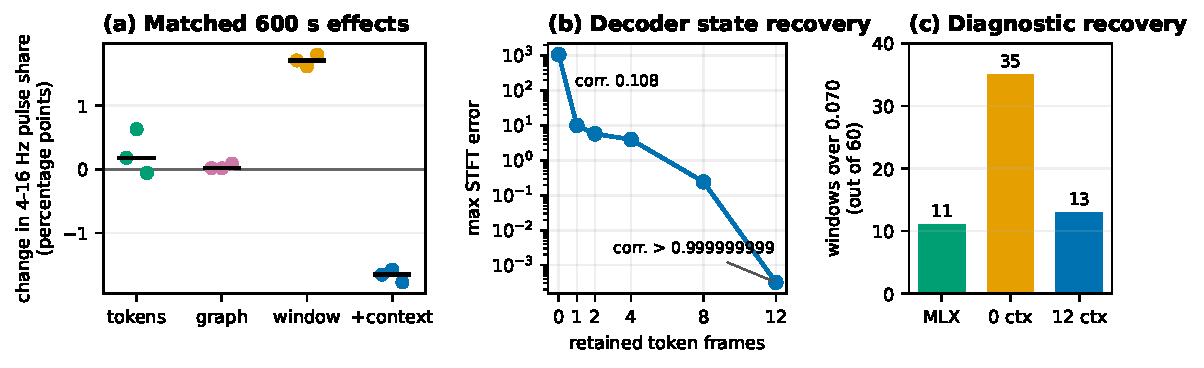
\includegraphics[width=\textwidth]{figures/fig-crossover.pdf}
  \caption{Causal localization. (a) Each dot is one 600 s seed; black bars are
  medians. (b) Twelve retained token frames recover stateful MLX pre-iSTFT
  output to correlation above 0.999999999. (c) The original prompt-specific
  0.070 diagnostic fires in 35/60 stateless Core ML windows, but only 13/60
  corrected windows versus 11/60 stateful MLX windows.}
  \label{fig:crossover}
\end{figure}

The crossover result is stable across all three seeds (\cref{tab:crossover}, \cref{fig:crossover}). Replacing MLX tokens with Core ML-port tokens at the stateful MLX decoder has median seed effect +0.00181, with range -0.00057 to +0.00627. Replacing the FLOAT32 MLX decoder graph with the FP16 Core ML graph under identical stateless windows and DSP has effect +0.00018 [0.00016, 0.00088]. Neither is large enough to explain the symptom.

Stateless windowing and the legacy production DSP, by contrast, add 0.01706 [0.01613, 0.01796] to pulse share relative to streaming MLX, and the paired difference is positive in all 60 windows. The FLOAT32 MLX graph reproduces the effect, exonerating FP16 as its primary source. Correcting the Hann convention without context adds another 0.00321 rather than removing it.

The context probe identifies the missing state. With no left history, a stateless 25-token evaluation has correlation 0.1083 with the corresponding stateful pre-iSTFT tensor and maximum absolute error 1,071.7. Correlation is 0.9926 with one token, 0.9999955 with eight, and above 0.999999999 with 12; maximum error falls to 0.000319. Under the same graph and corrected DSP, adding 12-token context reduces audio pulse share by 0.01650 [-0.01772, -0.01574], negative in all 60 paired windows.

The original 0.070 diagnostic fires in 35/60 stateless Core ML windows, 13/60 context-corrected windows, and 11/60 stateful MLX windows. On the physical A17 capture, median window share is 0.06091 and 5/20 windows cross the limit - exactly the stateful MLX count for seed 20260718. The final window is 0.09181, which reinforces why a single tail threshold is not a universal clock. The full trajectory contains no short exact token cycle, no sustained dropout, and no monotone decoder-specific late-onset failure.

The evidence therefore rejects the paper's earlier simple claim of runtime-independent long-horizon recurrence. It does not prove that MRT2 can never degenerate, or that every prompt is high quality. It proves that the measured pulse excess attributed to the phone path is caused primarily by an incorrect causal decoder boundary and is repaired by restoring measured history.

\subsection{Unrefreshed generation fails the frozen gate}

\begin{table}[H]
\centering
\small
\caption{Frozen 600 s unrefreshed liveness factorial. Entries are
float-PCM samples with $|x|\geq1.0$ (peak $|x|$). Reset arms intervene every
10 s while preserving RNG state and absolute position. Zero was required.
The factorial prevents overrange but does not identify a unique causal state.}
\label{tab:liveness}
\begin{tabular}{@{}lrrrr@{}}
\toprule
Seed & No reset & K/V only & Feedback only & Both \\
\midrule
20260718 & 2 (1.0028) & 0 (.9919) & 0 (.8616) & 0 (.9383) \\
271828   & 57 (1.1730) & 0 (.9264) & 13 (1.0359) & 0 (.8561) \\
1618033  & 46 (1.2382) & 0 (.9923) & 0 (.9923) & 0 (.9923) \\
\bottomrule
\end{tabular}
\end{table}

Every no-reset trajectory fails the zero-tolerance gate (\cref{tab:liveness}). The three seeds contain respectively 2, 57, and 46 float-PCM samples with \texttt{\detokenize{abs(x) >= 1.0}}, with peaks 1.0028, 1.1730, and 1.2382. All trajectories remain finite and none exhibits an exact short token cycle. The result is therefore a replicated full-scale-headroom failure for this configuration, not evidence of numerical explosion or proof that all of MRT2 is unusable.

Resetting both K/V and feedback prevents overrange in all three matched seeds. The factorial does not localize why. K/V-only also passes all three seeds; feedback-only passes two but leaves 13 overrange samples in seed 271828. Under the frozen classifier, one seed supports K/V-only rescue and two are ambiguous because multiple interventions land on the same safe side of a rare-event threshold. Aggregate attribution is therefore \textbf{ambiguous}, and no mitigation is promoted beyond the already-deployed combined reset.

All nine event-centered model lineups are control-valid: every reset baseline passes and every corrupted clip fails. The candidate is rejected in 7/9 votes, including 3/3 for seed 271828; these repeated calls are calibrated measurements, not independent listeners. In the separate blinded human check, the listener correctly rejects the corrupted clip but judges refreshed and unrefreshed clips both technically acceptable, noting only that the latter sounds "a little weird." That window covers seconds 570-600 and excludes the first measured overrange event. The evidence is consistent: the objective full-trajectory contract fails, while this one non-event human excerpt does not establish an audible failure.

The permitted conclusion is narrow: the tested no-reset, warm-prompt, 600-second configuration fails the frozen liveness gate in 3/3 seeds, and the reset-state attribution is unresolved. We neither call the model universally broken nor infer stable unrefreshed generation from acceptable excerpts.

\subsection{Post-ring steering fails after clean full delivery}
The first 600-second context-21 attempt at a 120 ms retained queue completes all 30 events but records seven underruns under sustained serious thermals and no detector-confirmed transition. A matched-noise context-21 diagnostic at a safer 200 ms queue eliminates delivery faults and detects all five measured changes, but end-to-end p95 is 0.790 seconds and maximum is 0.814 seconds, above the responsive gate. Context 23 reduces decoder emission to 40 ms but raises decoder call count enough to produce 165 underruns by the third calibration; the run is stopped.

The final corrected runtime instead uses five decoder input frames, two frames of causal history, a 120 ms emission quantum, and a 160 ms retained queue. Periodic refresh is disabled; each scripted event performs the matched reset. On the A17 Pro iPhone it completes 600 seconds and all 30 transitions, writes exactly 590 seconds of post-ring stereo PCM, and exits normally with zero underruns, producer drops, proof drops, or overflows. The runtime records a 1,024-frame (21.3 ms) low-water mark; the smallest end-of-iteration fill is 3,328 frames. All samples are finite, none reaches full scale, and peak magnitude is 0.999 after the safety clamp.

The four paired no-op windows freeze the detector threshold at 0.70249. Only 8/30 measured transitions cross it; 22 are missed. Among those eight detections, end-to-end p95 is 0.94675 seconds and maximum is 0.95120 seconds. Misses independently fail promotion, and the detected tail also exceeds the responsive limit. The frozen full protocol therefore fails both steering rungs and blocks the model-vote and physical-speaker tests.

This is a systems result, not evidence that text conditioning never affects MRT2. It establishes that the tested reset, decoder-cadence, and delivery protocol cannot jointly demonstrate responsive steering under its own false-change control. The supported product claim remains buffered playback.

\subsection{A14 is below the sustained boundary}
The A14 story remains a negative lower bound. Before the context repair, its certified FLOAT32 decoder configuration measured 43.88, 47.25, and 58.59 ms iteration-normalized p50/p90/p99, produced at 0.897x, and exhausted a 20.16 second reservoir after 294.08 seconds. It recorded 7,952 underruns. Context repair increases decoder cadence, so it cannot rescue this capacity result.

The A17 FP16 decoder artifact is not promoted on A14. A short ANE probe on A14 is finite but has unsafe amplitude; a long retry later becomes non-finite, while FLOAT32 CPU isolation remains bounded. We did not localize the exact overflowing layer, so we report a device-artifact numerical incompatibility, not a layer-level mechanism. A14 needs a different trained precision or decoder/depth architecture, not a larger hidden buffer.

\subsection{Compression ladder and early stopping}

\begin{figure}[H]
  \centering
  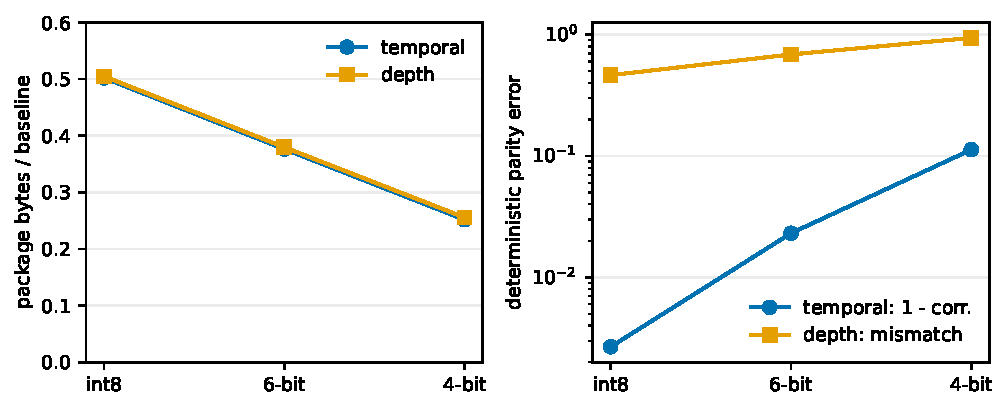
\includegraphics[width=0.94\textwidth]{figures/fig-compression.pdf}
  \caption{Rejected post-training compression ladder. Every artifact remains
  finite and becomes substantially smaller, but deterministic parity degrades
  monotonically. The gate order stops all six candidates before device timing
  or listening, avoiding a speed result for the wrong function.}
  \label{fig:compression}
\end{figure}

We also test int8 linear quantization and 6-bit and 4-bit palettization on temporal and depth packages (\cref{fig:compression}). Temporal packages shrink to 50.2\%, 37.6\%, and 25.2\% of baseline, but 64-step correlation falls to 0.9973, 0.9770, and 0.8874, below the 0.999 gate. Depth argmax mismatch reaches 46.3\%, 68.7\%, and 94.0\%. All remain finite; none reaches device timing. This is a negative result about tested post-training methods, not a claim that trained low-precision MRT2 is impossible.

\section{Discussion}
\subsection{Why the crossover changes the science}
The first manuscript had disciplined receipts and the wrong causal unit. It compared a 600-second phone capture with short clean MLX excerpts, then named a failed generative clock. The crossover forces every explanation to predict a path through fixed tokens. Because the FLOAT32 MLX pre-iSTFT graph reproduces the phone effect and 12-frame context cancels it under both graphs, the result is stronger than either "the model degenerates" or "Core ML is numerically different." It is a specific state-contract error with a minimal intervention.

This pattern generalizes. Causal neural decoders may expose a formal lookahead that is not their complete left-receptive-field contract. Exporting a static window without explicit state turns missing history into deterministic boundary modulation. Output finiteness, tensor shape parity, seam-jump metrics, and even short perceptual clips can all pass. A useful export test must compare a stateless window with a stateful prefix at multiple history depths.

\subsection{Fixing one boundary does not prove indefinite liveness}
The decoder crossover and unrefreshed factorial answer different causal questions. Restoring 12 frames of decoder history removes the deterministic 4-16 Hz boundary modulation. It cannot certify the autoregressive trajectory, because the principal crossover resets temporal state every ten seconds. The no-reset experiment closes that logical gap and fails its frozen headroom gate.

Conversely, a few float samples beyond nominal full scale do not retroactively prove that the original pulse was model recurrence. The stored signal is not integer-clipped, the human late-window check is acceptable, and reset arms sample different futures. The scientifically stable statement is the intersection: decoder history repairs the measured pulse defect; unrefreshed long-horizon generation still lacks a passing liveness certificate; combined ten-second reset is a bounded operating protocol whose causal mechanism remains unresolved.

\subsection{Throughput is not frame latency}
Dividing a batch time by 25 produces a unit of ms/token, not 25 observations. Its quantiles describe iteration-level compute density. They average away within-batch stalls and should not be labeled p99 frame latency. Our corrected compute clock uses the variable the architecture actually needs: sustained audio production relative to playback. Per-token tail latency would require instrumenting individual temporal/depth steps, which the current production log does not do.

This correction does not weaken the thermal result. The reservoir trajectory, producer rate, and late CPU+GPU-policy slowdown are batch-appropriate evidence. It does narrow the headline: we demonstrate sustained generation throughput, not a frame-synchronous 40 ms scheduler.

\subsection{Continuous playback is not interactive liveness}
A growing or high-watermark-limited reservoir prevents underflow and delays intent. The old delivery criterion accepted any final queue larger than the initial queue. For a continuously steerable model, that condition rewards the wrong behavior. A defensible upper bound is derived from prompt-change-to- audible-change latency, not memory capacity.

Post-ring evidence now sharpens that result. A 200 ms queue is clean but misses the responsive p95 gate, and a 40 ms decoder-emission configuration underruns. The final five-frame decoder closes delivery at a 160 ms queue for 600 seconds, but its frozen detector misses 22/30 changes and yields 0.947-second p95 among the detections. Because the objective full run fails, it is not promoted to the human speaker-level click test. The current system is therefore a robust buffered playback engine, not a demonstrated responsive or live engine.

\subsection{Evidence paths are systems too}
The project exposed two evidence-path bugs. An early recorder flattened a padded FP16 \texttt{\detokenize{MLMultiArray}}, manufacturing huge coefficients that live playback never consumed. The decoder's reconstruction core then used a different Hann convention from upstream. The first bug invalidated a capture; the second was a real parity debt but not the observed root cause. Both are now covered by independent stride-aware and sample-level tests.

The methodological rule is simple: test the measuring instrument with known good and known bad controls, then cross implementations before assigning a failure to the model. Hashes and manifests preserve evidence; they cannot make an underdetermined experiment causal.

\section{Limitations}
The crossover and reset factorial use three seeds and one ambient prompt. That is enough to replicate the decoder-boundary effect, not to characterize the prompt distribution or long-horizon musical quality of MRT2. The 4-16 Hz measure is prompt-sensitive and overlaps legitimate musical rhythm; its 0.070 value is reported only as the original diagnostic boundary. We do not use automated listening votes as independent statistical evidence. The nine event-centered calls are repeated measurements of one judge configuration, and the single blinded human engineering check is not a listening study. Its late window excludes the measured event. Neither instrument characterizes the prompt distribution or establishes population-level perceptual quality.

The MLX and Core ML token generators use different native random-number schemes. Token-source arms therefore test distributions and downstream symptoms, not token-exact port equivalence. Temporal fixtures and FLOAT32 depth rollout provide separate deterministic parity evidence, but rare FP16 near-tie flips remain expected. The context tensor probe uses one segment; three-seed full-audio interventions provide the broader replication.

The context-12 sustain runtime has one 610-second physical-device run, and the final five-frame steering runtime has one separate 600-second run. The placement campaign, pre-context latency campaign, and A14 study reuse prior signed builds with identical model artifacts; the context repair is host-only. The A14 FP16 failure is not localized to a layer. We report Instruments impact and placement evidence but no calibrated joules or battery-life claim.

Finally, steering is tested on one deliberately high-contrast prompt pair and 30 measured transitions in one device run. That is sufficient to reject promotion of this protocol, not to estimate steering quality over prompts or devices. No physical-speaker check was run after the objective failure, so the post-ring fade is not claimed click-free at the DAC or speaker. The raw WAVs, token captures, event traces, and device logs behind every table in this paper are public (see Artifact statement); the signed, compiled iOS application binary is not, and the generation runtime and render core are published as reference source rather than the shipping product.

\section{Conclusion}
MRT2 can sustain GPU-free generative-audio throughput on an A17 Pro iPhone under a ten-minute foreground thermal load. The corrected system produces at 1.030x nominal real time with zero underruns or drops, while a pure temporal boundary makes ANE admission repeatable. Those are substantial systems results, but they are not synonymous with per-token tail latency or low-latency steering.

The strongest result came from decomposing our own negative claim. A three-seed token-by-decoder crossover showed that an apparent long-horizon generative failure followed stateless decoder windowing, not the model, token source, FP16 graph, or Hann reconstruction. Twelve frames of measured causal history recover tensor parity and remove the excess on Mac and iPhone. Yet a separate no-reset protocol fails a frozen full-scale gate in all three seeds, and the reset factorial does not identify a unique responsible state. The honest deployed claim is therefore bounded: ten-second reset, sustained throughput, and buffered playback. The final post-ring steering run closes delivery but fails its acoustic promotion gate. Live generation has three clocks. Good science requires measuring each one, preserving negative results, and refusing to let a repair on one clock certify another.

\section{Artifact statement}
The public repository, \texttt{\detokenize{github.com/mattmireles/magenta-realtime-2-iphone}}, contains Core ML exporters, frozen fixtures, placement and sustain verifiers, the three 600-second crossover reports, decoder-context probe, corrected A17 normalized manifest, compression ladder, figure sources, paper source, and exact build protocol. It additionally contains, under \texttt{\detokenize{harness/}}, the generation/decode/summarize/probe scripts referenced in Reproducibility as "the Crossfade harness," and, under \texttt{\detokenize{harness/reference-runtime/}}, the exact source of the producer-loop runtime and the C++ inverse-STFT render core that produced the corrected A17 sustained-throughput run, each verifiable against the \texttt{\detokenize{generationRuntimeSourceSha256}} / \texttt{\detokenize{renderCoreSourceSha256}} fields in \texttt{\detokenize{context12-soak-manifest.json}}.

The raw evidence itself, every WAV, token capture, event trace, and device log hashed by a manifest in \texttt{\detokenize{validation/results/system-paper/}}, is public as release assets at \texttt{\detokenize{github.com/mattmireles/magenta-realtime-2-iphone}} / \texttt{\detokenize{releases/tag/evidence-v1}} (139 files, individually sha256-verified against the manifests both before and after upload). The mapping from each published hash to its public asset is \texttt{\detokenize{evidence/evidence-manifest.json}} and \texttt{\detokenize{evidence/release-asset-map.json}} in the repository. A Hugging Face dataset mirror can be published from the same verified manifest via \texttt{\detokenize{evidence/publish_to_huggingface.py}}. Two things remain private: the signed, compiled iOS application binary (\texttt{\detokenize{signedExecutableSha256}} records its hash but not its bytes), and the single blinded human engineering listening check, which was never machine-hash-bound and is reported only as prose in Limitations.

\section{Acknowledgments}
OpenAI Codex assisted with experimental code, data normalization, figure generation, and manuscript preparation. The author designed the study, operated the devices, inspected the evidence, selected the claims, and accepts responsibility for the manuscript.

\appendix
\section{Reproducibility}
\subsection{Public evidence map}
The canonical crossover result is \texttt{\detokenize{aggregate.json}} in the public crossover receipt directory. It hashes three seed reports and the decoder-context probe. Each seed report hashes token summaries and every decoded WAV arm. The corrected physical-device receipt is \texttt{\detokenize{context12-soak-manifest.json}} in the A17 context-12 directory; it hashes the 600-second PCM capture, 610-second event trace, 15,790-frame token capture, normalized summaries, signed executable, runtime source, and render core source. Every one of these hashed files, the raw WAVs, token captures, and event traces, not only their summaries, is public as release assets at \texttt{\detokenize{github.com/mattmireles/magenta-realtime-2-iphone}} / \texttt{\detokenize{releases/tag/evidence-v1}}; the exact source-to-hash mapping is \texttt{\detokenize{evidence/evidence-manifest.json}} and \texttt{\detokenize{evidence/release-asset-map.json}} in the repository. The three seed-report JSON files themselves retain the original authoring machine's local file paths in their \texttt{\detokenize{path}} fields: those files are individually hash-bound by \texttt{\detokenize{aggregate.json}}, so editing them to remove the local paths would invalidate a hash already published as a scientific receipt. The public dataset mapping resolves each local path to its public counterpart without touching the receipts.

The unrefreshed result is \texttt{\detokenize{validation/results/system-paper/liveness/g5-manifest.json}}. It records the frozen gate, all 12 factorial arms, reset counters, candidate and control vote outcomes, permitted claim, and hashes of tokens, WAVs, lineups, vote reports, protocol, index, and analysis, all of which are public in the same evidence dataset. The public verifier treats the failed G5 status as a valid scientific result and rejects missing seeds, changed thresholds, invalid controls, machine-local paths, or broader wording.

The steering result is \texttt{\detokenize{validation/results/system-paper/steering/g6-manifest.json}}. It binds the post-ring WAV, event trace, tokens, detector reports, device identity, signed executable, and exact buffered-only wording. Every artifact except the signed executable is public in the same dataset. The verifier accepts this complete 600-second negative result but requires all 30 transitions to be detected inside a latency rung, plus calibrated listening and a physical-speaker record, to promote a responsive or live claim.

The A17 and A14 placement directories contain admission receipts. The historical A17 placement soak and CPU+GPU duration control are under \texttt{\detokenize{a17pro/soak/}} and \texttt{\detokenize{evaluation/}}. The A14 bounded-reservoir result is under \texttt{\detokenize{a14/soak/}}. \texttt{\detokenize{MRT2WeightCompressionLadder.json}} contains all six early-stopped compression arms, and \texttt{\detokenize{depth-rollout-ablation.json}} records the measured 12-call, one-call FLOAT32, and one-call FLOAT16 depth results.

\subsection{Crossover commands}
The Crossfade harness, published under \texttt{\detokenize{harness/}} in the repository, exposes generation, decoding, summarization, and decoder-context probe subcommands as \texttt{\detokenize{run_mrt2_long_horizon_crossover.py}}, \texttt{\detokenize{probe_spectrostream_rvq_lookup.py}}, and related scripts (see \texttt{\detokenize{harness/README.md}} for the full command-to-section map). A complete replication uses 15,001 codebook-local token frames, temperature 1.0, top-k 40, a 10-second refresh, and a 600-second decode. Decoder arms name the token file explicitly; the analyzer refuses incomplete fixed-DSP or context pairs. Running the harness end to end additionally requires the converted model artifacts and compiled render core described in §3.3; the render core's exact source is \texttt{\detokenize{harness/reference-runtime/RenderCore.cpp}}.

The public analysis commands are:

\begin{itemize}
\item run \texttt{\detokenize{analyze_system_paper_crossover.py}} once per seed with the four 2x2 WAVs, FLOAT32 graph split, four corrected-DSP controls, and two context arms;
\item run \texttt{\detokenize{aggregate_system_paper_crossover.py}} on the three reports plus \texttt{\detokenize{decoder-context-probe.json}}; and
\item regenerate \texttt{\detokenize{fig-crossover.pdf}} from the aggregate only.
\end{itemize}
\subsection{Unrefreshed liveness verification}
Run \texttt{\detokenize{validation/verify_system_paper_liveness.py}} with the public G5 manifest and the physical-device G6 steering manifest. The G5 branch requires exactly three seeds and four reset arms, verifies that no-reset fails in 3/3 and combined reset passes in 3/3, preserves the ambiguous attribution, validates all nine listening controls, and enforces the narrow permitted claim.

\subsection{Corrected runtime protocol}
\begin{enumerate}
\item Load the signed precompiled models with explicit compute policies, query the temporal compute plan, execute the fresh/warmed state proof, and perform three untimed warmups.
\item Prime the PCM ring. For each token frame, present chronological temporal K/V, run one temporal prediction, sample 12 depth levels in one prediction, and sum selected RVQ rows.
\item Once 25 decoder embeddings are available, predict 96 STFT frames. After the first window, retain 12 token embeddings, advance by 12, discard 48 context STFT frames, and send only 48 new frames to the periodic-Hann inverse STFT.
\item Push PCM off the callback. The callback performs bounded ring reads; count zero-fill underruns. Backpressure at the high watermark. Every 10 seconds, clear temporal K/V and previous feedback without clearing decoder context, overlap-add state, or queued PCM.
\item Capture logical STFT-derived PCM and codebook-local tokens independently; stop after 610 seconds and hash every artifact before normalization.
\end{enumerate}
\subsection{Verification suites}
The public suites cover crossover audio analysis, seed aggregation, G1-G4 manifests, placement, sustain, and compression contracts. The private runtime suites cover Swift configuration defaults, padded \texttt{\detokenize{MLMultiArray}} reads, exact SplitMix64 Gumbel values, cache updates, token-cycle metrics, C++ periodic-Hann sample parity, and the signed iOS build. Tectonic rebuilds the paper from the readable Markdown source, and Poppler-rendered pages are visually audited before publication.

\bibliographystyle{plainnat}
\bibliography{refs}
\end{document}
